\section{Instellingen}


\subsection{Vertalen}
\pvelist{ \pve{2.10} }
Alle teksten die in de website worden gebruikt en geen deel uitmaken van de paginainhoud kunnen worden vertaald via de Drupal vertaalinterface. Deze interface is beschikbaar op \emph{Instellingen} $\rightarrow$ \emph{Interface vertalen} of direct op \drupalpath{admin/config/regional/translate}. Klik op het tabblad \emph{Vertalen}.

Via het formulier bovenin kan worden gezocht naar teksten op de website. Vul hiervoor (een deel van) de tekst in die vertaald moet worden. Deze zoekfunctionaliteit is hoofdlettergevoelig.

Klik in de lijst van teksten op \emph{bewerken} om een vertaling in te voeren.

\subsection{Calamiteiten pagina}
\pvelist{ \pve{4.1.1.2, 4.4} }
Om de site in calamiteiten mode te zetten ga je als volgt te werk:

\begin{enumerate}
\item Ga naar \drupalpath{node/237/edit} om de calamiteiten pagina te bewerken indien nodig
\item Controleer of de calamiteitenpagina is gepubliceerd
\item Ga naar \emph{Structuur} $\rightarrow$ \emph{Dominion} of direct naar \drupalpath{admin/structure/dominion/list/1/edit}
\item Vul bij \emph{voorpagina} de tekst \emph{calamiteiten} in
\item Klik op Oplaan
\end{enumerate}

Op de calamiteitenpagina heeft de redacteur alle vrijheid om blokken te plaatsen, net zoals alle andere pagina's.

\begin{figure}[p]
\centering
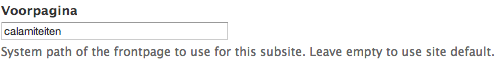
\includegraphics[width=\textwidth]{img/calamiteiten.png}
\caption{Calamiteiten pagina activeren}
\label{fig:calamiteiten_image}
\end{figure}


%your config here
\newcommand{\projectname}{WIM Release 1.15}

\newcommand{\customer}{Dimpact} %let op spatie 
\newcommand{\customershort}{HK} %let op spatie

\newcommand{\customerdomain}{bdu.nl}
\newcommand{\authors}{BS Meijer - R Meijer}
\newcommand{\doprep}{BS Meijer - R Meijer}
\newcommand{\customerrep}{J Donkers } %let op spatie
\newcommand{\offerdate}{11-03-2016}
\newcommand{\leaddate}{10-03-2016 } %let op spatie
\newcommand{\runtime}{4 weken } %let op spatie
\newcommand{\lastversion}{1.0}
\newcommand{\lastupdate}{24-03-2016}

\begin{document}
\ThisLRCornerWallPaper{0.8}{assets/img/voorbladlogo.png}

\title{\textbf{\customer} \\ \projectname}
\pretitle{\begin{flushleft}\LARGE}
\posttitle{\par\end{flushleft}}

% The actual Document:
\author{}
\date{}

\maketitle

\vspace{-2.6cm}
\begin{flushright}
\begin{tabularx}{4.8cm}{ X }
Dutch Open Projects			\\
Doornseweg 12					\\	
3832 RL Leusden					\\
T: +31[0]33 - 4 50 50 50		\\
F: +31[0]33 - 4 50 50 57		
\\*
\\*
\\*
\\*
\\*
\\*
\\*
\\*
\\*
\\*
\\*
\\*
\\*
\\*
\\*
\\*
\\*
\\*
\footnotesize
All rights reserved.\\*
\footnotesize
No part of the contents of this publication may be reproduced, stored in a data processing system or transmitted in any form or by any means without the written permission of Dutch Open Projects B.V.
\end{tabularx}
\end{flushright}
  
 \null
 \vfill    
  \begin{tabularx}{\linewidth}{ p{4cm} X }
    Plaats & Leusden								\\
    Laatst bijgewerkt & \lastupdate		\\
    Auteurs & \authors							\\
    Versie & \lastversion			\\
  \end{tabularx}
\pagebreak

\URCornerWallPaper{0.13}{assets/img/koptekstlogo.png}

\section*{Copyright}
\textcopyright  2016 Dutch Open Projects \\
Alle rechten voorbehouden

\pagebreak
\section*{Versie- \& Distributiehistorie}
\subsection*{Versiehistorie}
\begin{tabularx}{\linewidth} { | l | l | l | X |} \hline
\textbf{Versie} & \textbf{Datum} & \textbf{Auteur} & \textbf{Omschrijving} \\ \hline
1.0 & 24-03-2016 & BS Meijer, R Meijer & - \\ \hline
\end{tabularx}

\subsection*{Distributiehistorie}
\begin{tabularx}{\linewidth} { | l | l | l | X |} \hline
\textbf{Versie} & \textbf{Datum} & \textbf{Auteur} & \textbf{Gedistribueerd aan} \\ \hline
1.0 & 24-03-2016 & BS Meijer, R Meijer & DOP Repository, Dimpact \\ \hline
\end{tabularx}
\clearpage

\include{assets/tableofcontents}
\tableofcontents
\pagebreak

\section{Release 1.15}
De release 1.15 bestaat uit de volgende onderdelen:
\subsection{Merges uit Git}
Vanuit Git zijn de volgende 5 pullrequests doorgekomen in WIM. Deze zijn door Dimpact beoordeeld zijn in onderdeel uitmaken van release 1.15. Voor pullrequest 5 en 6 zijn opmerkingen, deze zijn onder de tabel te lezen.

\begin{tabularx}{\linewidth}{l|l|X} \hline
PullReq. & Release & Opmerking \\ \hline
10 & 1.15 & Add RSS feed from enschede \\ \hline
9 & 1.15 & Add Mylex C-content integration and add created and modify date to custom lists
and fix double statement end \\ \hline
7 & 1.15 & Media in WYSIWYG adds empty tags, remove those with a hook \\ \hline
6 & 1.15 & Custom Twitter module that allows creating Tweet blocks and filtering on words * \\ \hline
5 & 1.15 & Add additional wrapper/container divs + add two meta menus to the footer ** \\ \hline
\end{tabularx}

* Dit is een custom module die aangezet kan worden door de implementator \\
** In deze request hebben wij een aanpassing gemaakt, omdat hij anders bestaande functionaliteit van WIM zou breken inzake de menustructuur in de footer. Zie ticket \#738 in de Dimpact SLA in Unfuddle, het betreft het volgende comment:

\textit{Pull request 'Add additional wrapper/container divs + add two meta menus to the footer' is aangepast, zodat bestaande menu's niet worden verwijderd.
}

\textit{Het gaat om:}
\begin{enumerate}
\item menu-footer-menu (Direct online regelen2)
\item menu-meta-menu-links-intranet (Meta menu links intranet)
\end{enumerate}

\subsubsection{Niet opgenomen mergerequests}
De volgende pullrequests zijn niet opgenomen in release 1.15:

\begin{tabularx}{\linewidth}{l|l|X} \hline
PullReq. & Release & Opmerking \\ \hline
8 & - & Disable tags display on news and pages content type \\ \hline
\end{tabularx}

De pullrequest is niet opgenomen omdat deze teveel consequenties heeft voor de huidige implementaties.

\subsection{Security Updates}
Voor release 1.15 zijn de volgende onderdeel gepatched inzake security updates:

\begin{tabularx}{\linewidth}{X|l|l} \hline
Onderdeel & Vorige versie & Nieuwe versie \\ \hline
Drupal Core & 7.41 & 7.43 \\ \hline
\end{tabularx}

\subsection{Module updates}
De volgende modules zijn ge\"updatet in release 1.15:

\begin{tabularx}{\linewidth}{X|l|l} \hline
Onderdeel & Vorige versie & Nieuwe versie \\ \hline
\texttt{apachesolr\_exclude\_node} & 1.1 & 1.4 \\ \hline
\texttt{email} & 1.2 & 1.3 \\ \hline
\texttt{extlink} & 1.13 & 1.18 \\ \hline
\texttt{fences} & 1.0 & 1.2 \\ \hline
\texttt{xmlsitemap} & 2.0 & 2.2 \\ \hline
\end{tabularx}

\subsection{Changes}
Onderstaande tabel geeft aan op welke punten het moedersjabloon functioneel is gewijzigd. Gebruikers van het systeem moeten er rekening mee houden dat het product op

deze punten anders werkt dan voorheen.De volgende changes zijn doorgevoerd in release 1.15:

\begin{tabularx}{\linewidth}{l|l|X} \hline
Ticket & Release & Opmerking \\ \hline
594 & 1.15 & Meerdere bestanden tegelijk uploaden/wissen op /admin/workbench/file/add \\ \hline
690 & 1.15 & Readspeaker: docreader ook implementeren \\ \hline
\end{tabularx}

\subsection{Bundler}
Voor de implementatiepartners is de volgende change doorgevoerd. We hebben een bundler config toegevoegd aan het systeem.

Het 'phing theme'-commando is onafhankelijk gemaakt van Bundler, als Bundler niet is ge\"installeerd dan wordt gewoon de huidige manier van compileren gebruikt (via compass), als Bundler wel is ge\"installeerd \'en 'bundle install' is gedraaid om de juiste gems op te halen, dan wordt Bundler gebruikt om de CSS te compileren.

\section{Testresultaten}
De geleverde versie bevat geen known issues.
\end{document}
